\PassOptionsToPackage{xcolor}{usenames,dvipsnames,svgnames,table}
\documentclass[10pt]{report}
\usepackage[T1]{fontenc}
\usepackage{lmodern}
\usepackage{pdfcolmk}
\usepackage{multirow}
\usepackage{graphicx}
\usepackage{pifont}
\usepackage{amsmath,amsfonts,amsthm,amssymb}
\usepackage{setspace}
\usepackage{Tabbing}
\usepackage{etoolbox}
\usepackage{fancyhdr}
\usepackage{lastpage}
\usepackage{listings}
\usepackage{extramarks}
\usepackage{enumerate}
\usepackage{soul,color}
\usepackage{graphicx,float,wrapfig}
\usepackage{amsmath,amssymb,rotating}
\usepackage{epsfig}
\usepackage{color}
\usepackage{hyperref}
\usepackage{animate}
\usepackage{array}
\usepackage{graphics, color}
\usepackage{graphicx}
\usepackage{epsfig}
\usepackage{setspace}
\usepackage{verbatim}
\usepackage[margin=1.0in]{geometry}
\usepackage{tikz}
\usepackage{mdframed}
\usepackage{clrscode3e}
\usepackage{formalHW}
\usepackage[none,DMC]{formatHW}
\usepackage{fancyquote}
\usepackage{fancyenvironments}
\usepackage{mymathmacros}
\usepackage{algorithm}
\usepackage[noend]{algpseudocode}
\usepackage{pgfplots}

%set up fancy page header
\pagestyle{fancy}
   \chead{DMC@ISU:\ Too many features}  
   \rhead{\firstxmark}
   \lfoot{\lastxmark}
   \cfoot{}
   \rfoot{Page\ \thepage\ of\ \pageref{LastPage}}
   \renewcommand\headrulewidth{0.4pt}
   \renewcommand\footrulewidth{0.4pt}

% pandoc syntax highlighting
\usepackage{color}
\usepackage{fancyvrb}
\newcommand{\VerbBar}{|}
\newcommand{\VERB}{\Verb[commandchars=\\\{\}]}
\DefineVerbatimEnvironment{Highlighting}{Verbatim}{commandchars=\\\{\}}
% Add ',fontsize=\small' for more characters per line
\newenvironment{Shaded}{}{}
\newcommand{\KeywordTok}[1]{\textcolor[rgb]{0.00,0.44,0.13}{\textbf{{#1}}}}
\newcommand{\DataTypeTok}[1]{\textcolor[rgb]{0.56,0.13,0.00}{{#1}}}
\newcommand{\DecValTok}[1]{\textcolor[rgb]{0.25,0.63,0.44}{{#1}}}
\newcommand{\BaseNTok}[1]{\textcolor[rgb]{0.25,0.63,0.44}{{#1}}}
\newcommand{\FloatTok}[1]{\textcolor[rgb]{0.25,0.63,0.44}{{#1}}}
\newcommand{\CharTok}[1]{\textcolor[rgb]{0.25,0.44,0.63}{{#1}}}
\newcommand{\StringTok}[1]{\textcolor[rgb]{0.25,0.44,0.63}{{#1}}}
\newcommand{\CommentTok}[1]{\textcolor[rgb]{0.38,0.63,0.69}{\textit{{#1}}}}
\newcommand{\OtherTok}[1]{\textcolor[rgb]{0.00,0.44,0.13}{{#1}}}
\newcommand{\AlertTok}[1]{\textcolor[rgb]{1.00,0.00,0.00}{\textbf{{#1}}}}
\newcommand{\FunctionTok}[1]{\textcolor[rgb]{0.02,0.16,0.49}{{#1}}}
\newcommand{\RegionMarkerTok}[1]{{#1}}
\newcommand{\ErrorTok}[1]{\textcolor[rgb]{1.00,0.00,0.00}{\textbf{{#1}}}}
\newcommand{\NormalTok}[1]{{#1}}

% header includes

\begin{document}

\thispagestyle{empty}%
\begin{center}%
    \renewcommand{\arraystretch}{1.5}%
    \begin{tabular}{c}%
       \Large{DMC@ISU: The 2015 Iowa State University Data Mining Cup Team}\\
       Curation and Cross Validation to Reduce Features\\
       Spring 2015, A Team as Strong as Steel \\
    \end{tabular}
\end{center}

\begin{center}
 \renewcommand{\arraystretch}{1.5}
 \begin{tabular*}{0.65\textwidth}{r@{:\hspace{.3cm}}l}
    \hline
    
    
    Last Day&  May 19, 2015\\
    \hline
 \end{tabular*}
\end{center}

I am using the following packages:

\begin{Shaded}
\begin{Highlighting}[]
   \KeywordTok{library}\NormalTok{(magrittr)}
   \KeywordTok{library}\NormalTok{(dplyr)}
   \KeywordTok{library}\NormalTok{(reshape2)}
   \KeywordTok{library}\NormalTok{(tidyr)}
   \KeywordTok{library}\NormalTok{(lubridate)}
   \KeywordTok{library}\NormalTok{(ggplot2)}
   \KeywordTok{library}\NormalTok{(gridExtra)}
   \KeywordTok{library}\NormalTok{(directlabels)}
   \KeywordTok{library}\NormalTok{(rCharts)}
   \KeywordTok{library}\NormalTok{(xtable)}
   \KeywordTok{library}\NormalTok{(foreach)}
   \KeywordTok{library}\NormalTok{(gtools)}
   \KeywordTok{library}\NormalTok{(knitr)}
   \KeywordTok{library}\NormalTok{(utils)}
   \KeywordTok{library}\NormalTok{(GGally)}
   \KeywordTok{source}\NormalTok{(}\StringTok{"~/dmc2015/ian/R/renm.R"}\NormalTok{)}
\end{Highlighting}
\end{Shaded}

\begin{Shaded}
\begin{Highlighting}[]
\NormalTok{predPlot =}\StringTok{ }\NormalTok{function(pred_set1, pred_set2) \{}
    \NormalTok{p =}\StringTok{ }\KeywordTok{qplot}\NormalTok{(pred_set1, pred_set2) +}\StringTok{ }\KeywordTok{coord_fixed}\NormalTok{() +}\StringTok{ }\KeywordTok{geom_abline}\NormalTok{(}\DataTypeTok{intercept =} \DecValTok{0}\NormalTok{, }
        \DataTypeTok{slope =} \DecValTok{1}\NormalTok{, }\DataTypeTok{color =} \StringTok{"red"}\NormalTok{)}
    \KeywordTok{print}\NormalTok{(p)}
    \KeywordTok{return}\NormalTok{(p)}
\NormalTok{\}}

\NormalTok{lossFunction =}\StringTok{ }\NormalTok{function(pred, actual) }\KeywordTok{sum}\NormalTok{(((}\DecValTok{1}\NormalTok{/}\KeywordTok{mean}\NormalTok{(actual)) *}\StringTok{ }\NormalTok{(pred -}\StringTok{ }\NormalTok{actual))^}\DecValTok{2}\NormalTok{)}

\NormalTok{predictor_weight =}\StringTok{ }\NormalTok{function(pred1, pred2, actual) \{}
    \NormalTok{alphas =}\StringTok{ }\KeywordTok{seq}\NormalTok{(}\DecValTok{0}\NormalTok{, }\DecValTok{1}\NormalTok{, }\FloatTok{0.001}\NormalTok{)}
    \NormalTok{err =}\StringTok{ }\KeywordTok{sapply}\NormalTok{(alphas, function(alpha) }\KeywordTok{lossFunction}\NormalTok{(alpha *}\StringTok{ }\NormalTok{pred1 +}\StringTok{ }\NormalTok{(}\DecValTok{1} \NormalTok{-}\StringTok{ }\NormalTok{alpha) *}\StringTok{ }
\StringTok{        }\NormalTok{pred2, actual))}
    \NormalTok{pred =}\StringTok{ }\KeywordTok{data.frame}\NormalTok{(}\DataTypeTok{proportion.1 =} \NormalTok{alphas, }\DataTypeTok{err =} \NormalTok{err)}
    \KeywordTok{return}\NormalTok{(pred)}
\NormalTok{\}}
\end{Highlighting}
\end{Shaded}

My working directory is set to \verb!~/dmc2015/predictions/!.

\section{Set 1}\label{set-1}

I am using our new clean data - so should you

\begin{Shaded}
\begin{Highlighting}[]
\KeywordTok{source}\NormalTok{(}\StringTok{"~/dmc2015/ian/load_data.r"}\NormalTok{)}
\end{Highlighting}
\end{Shaded}

\begin{verbatim}
## using the following as id:
##  orderID,
##  orderTime,
##  userID,
##  couponsReceived,
##  basketValue,
##  couponsReceivedDate,
##  couponsReceivedTime,
##  couponsReceivedDoW,
##  couponsReceivedWeekend,
##  couponsReceivedFriSat,
##  orderTimeDate,
##  orderTimeTime,
##  orderTimeDoW,
##  orderTimeWeekend,
##  orderTimeFriSat,
##  batchID,
##  couponsExpire,
##  couponsSent,
##  TimeBtwnSentRec,
##  TimeBtwnRecExpire,
##  TimeBtwnRecOrder,
##  TimeBtwnOrderExpire,
##  ShopFast,
##  EarlyRec,
##  Shop60,
##  Shop30,
##  Shop15,
##  RecExpire60,
##  RecOrder60,
##  OrderExpire60
## 
## using the following as measure columns:
##  couponID1,
##  price1,
##  basePrice1,
##  reward1,
##  premiumProduct1,
##  brand1,
##  productGroup1,
##  categoryIDs1,
##  coupon1Used,
##  basePrice_price_ratio1,
##  couponID2,
##  price2,
##  basePrice2,
##  reward2,
##  premiumProduct2,
##  brand2,
##  productGroup2,
##  categoryIDs2,
##  coupon2Used,
##  basePrice_price_ratio2,
##  couponID3,
##  price3,
##  basePrice3,
##  reward3,
##  premiumProduct3,
##  brand3,
##  productGroup3,
##  categoryIDs3,
##  coupon3Used,
##  basePrice_price_ratio3
\end{verbatim}

\begin{Shaded}
\begin{Highlighting}[]
\NormalTok{HTVset1 =}\StringTok{ }\KeywordTok{readRDS}\NormalTok{(}\StringTok{"~/dmc2015/data/featureMatrix/HTVset1.rds"}\NormalTok{)}
\NormalTok{actual.val =}\StringTok{ }\KeywordTok{as.vector}\NormalTok{(}\KeywordTok{t}\NormalTok{(HTVset1$V[, }\KeywordTok{c}\NormalTok{(}\StringTok{"coupon1Used"}\NormalTok{, }\StringTok{"coupon2Used"}\NormalTok{, }\StringTok{"coupon3Used"}\NormalTok{)]))}
\end{Highlighting}
\end{Shaded}

\subsection{Reading in the
predictions}\label{reading-in-the-predictions}

The predictions are stored in \verb!~/dmc2015/predictions/!. We can read
the files into R using the \verb!list.files! function.

\begin{Shaded}
\begin{Highlighting}[]
\NormalTok{files =}\StringTok{ }\KeywordTok{list.files}\NormalTok{(}\StringTok{"~/dmc2015/predictions/set1/"}\NormalTok{, }\DataTypeTok{pattern =} \StringTok{"rds"}\NormalTok{, }\DataTypeTok{full.names =} \OtherTok{TRUE}\NormalTok{)}
\NormalTok{files}
\end{Highlighting}
\end{Shaded}

\begin{verbatim}
##  [1] "/Users/user/dmc2015/predictions/set1//crf_386col_set1_0.8.rds"
##  [2] "/Users/user/dmc2015/predictions/set1//crf_ada_set1_0.3.rds"   
##  [3] "/Users/user/dmc2015/predictions/set1//crf_c50_set1_0.3.rds"   
##  [4] "/Users/user/dmc2015/predictions/set1//crf_c50_set1_0.4.rds"   
##  [5] "/Users/user/dmc2015/predictions/set1//crf_crf_set1_0.3.rds"   
##  [6] "/Users/user/dmc2015/predictions/set1//crf_crf_set1_0.5.rds"   
##  [7] "/Users/user/dmc2015/predictions/set1//crf_lasso_set1_0.3.rds" 
##  [8] "/Users/user/dmc2015/predictions/set1//crf_lasso_set1_0.4.rds" 
##  [9] "/Users/user/dmc2015/predictions/set1//crf_rf_set1_0.3.rds"    
## [10] "/Users/user/dmc2015/predictions/set1//crf_rf_set1_0.4.rds"    
## [11] "/Users/user/dmc2015/predictions/set1//gbm_386col_set1_0.8.rds"
## [12] "/Users/user/dmc2015/predictions/set1//gbm_rf_set1_0.8.rds"    
## [13] "/Users/user/dmc2015/predictions/set1//lasso_386col_set1.rds"  
## [14] "/Users/user/dmc2015/predictions/set1//lasso_c50_set1.rds"     
## [15] "/Users/user/dmc2015/predictions/set1//lasso_crf_set1.rds"     
## [16] "/Users/user/dmc2015/predictions/set1//lasso_gbm_set1.rds"     
## [17] "/Users/user/dmc2015/predictions/set1//lasso_lasso_set1.rds"   
## [18] "/Users/user/dmc2015/predictions/set1//lasso_rf_set1.rds"      
## [19] "/Users/user/dmc2015/predictions/set1//pca_386col_set1.rds"    
## [20] "/Users/user/dmc2015/predictions/set1//pca_c50_set1.rds"       
## [21] "/Users/user/dmc2015/predictions/set1//pca_crf_set1.rds"       
## [22] "/Users/user/dmc2015/predictions/set1//pca_gbm_set1.rds"       
## [23] "/Users/user/dmc2015/predictions/set1//pca_lasso_set1.rds"     
## [24] "/Users/user/dmc2015/predictions/set1//pca_rf_set1.rds"        
## [25] "/Users/user/dmc2015/predictions/set1//rf_386col_set1.rds"     
## [26] "/Users/user/dmc2015/predictions/set1//rf_c50_set1.rds"        
## [27] "/Users/user/dmc2015/predictions/set1//rf_lasso_set1.rds"      
## [28] "/Users/user/dmc2015/predictions/set1//rf_rf_set1.rds"
\end{verbatim}

\begin{Shaded}
\begin{Highlighting}[]
\CommentTok{# base names}
\NormalTok{base_names =}\StringTok{ }\KeywordTok{gsub}\NormalTok{(}\StringTok{"(/Users/user/dmc2015/predictions/set1//)(.*)(}\CharTok{\textbackslash{}\textbackslash{}}\StringTok{.rds)"}\NormalTok{, }\StringTok{"}\CharTok{\textbackslash{}\textbackslash{}}\StringTok{2"}\NormalTok{, }
    \NormalTok{files)}
\end{Highlighting}
\end{Shaded}

Many of the sets have the \textbf{DMC Official} structure:

\begin{Shaded}
\begin{Highlighting}[]
\NormalTok{DMCofficial =}\StringTok{ }\KeywordTok{readRDS}\NormalTok{(}\StringTok{"~/dmc2015/predictions/set1/crf_386col_set1_0.8.rds"}\NormalTok{)}
\KeywordTok{str}\NormalTok{(DMCofficial)}
\end{Highlighting}
\end{Shaded}

\begin{verbatim}
## List of 4
##  $ val_predictions  : num [1:4035, 1] 0.208 0.245 0.217 0.252 0.193 ...
##   ..- attr(*, "dimnames")=List of 2
##   .. ..$ : NULL
##   .. ..$ : chr "couponUsed"
##  $ class_predictions: num [1:2007, 1:2] 6054 6054 6054 6055 6055 ...
##   ..- attr(*, "dimnames")=List of 2
##   .. ..$ : NULL
##   .. ..$ : chr [1:2] "orderID" "couponUsed"
##  $ error            : num [1:4] 3931 5985 6463 16379
##  $ details          :List of 4
##   ..$ vars  : chr "Peng Liahua's variables"
##   ..$ nvars : num 386
##   ..$ ntrees: num 1000
##   ..$ mtry  : num 10
\end{verbatim}

I can check the structure in a similar way to how I read in features:

\begin{Shaded}
\begin{Highlighting}[]
\NormalTok{preds =}\StringTok{ }\KeywordTok{lapply}\NormalTok{(files, function(x) }\KeywordTok{readRDS}\NormalTok{(x))}
\NormalTok{pred.struc =}\StringTok{ }\KeywordTok{rep}\NormalTok{(}\StringTok{"renegade style"}\NormalTok{, }\KeywordTok{length}\NormalTok{(files))}

\NormalTok{for (i in }\DecValTok{1}\NormalTok{:}\KeywordTok{length}\NormalTok{(files)) \{}
    \NormalTok{if (}\KeywordTok{all}\NormalTok{(}\KeywordTok{names}\NormalTok{(preds[[i]]) %in%}\StringTok{ }\KeywordTok{names}\NormalTok{(DMCofficial))) \{}
        \NormalTok{pred.struc[i] =}\StringTok{ "DMC Official"}
    \NormalTok{\}}
\NormalTok{\}}

\NormalTok{pred.struc}
\end{Highlighting}
\end{Shaded}

\begin{verbatim}
##  [1] "DMC Official"   "DMC Official"   "DMC Official"   "DMC Official"  
##  [5] "DMC Official"   "DMC Official"   "DMC Official"   "DMC Official"  
##  [9] "DMC Official"   "DMC Official"   "renegade style" "renegade style"
## [13] "renegade style" "renegade style" "renegade style" "renegade style"
## [17] "renegade style" "renegade style" "renegade style" "renegade style"
## [21] "renegade style" "renegade style" "renegade style" "renegade style"
## [25] "renegade style" "renegade style" "renegade style" "renegade style"
\end{verbatim}

We can get the DMC official \textbf{validation predictions} like this:

\begin{Shaded}
\begin{Highlighting}[]
\CommentTok{# which files were DMC Official?}
\NormalTok{these_ones =}\StringTok{ }\KeywordTok{which}\NormalTok{(pred.struc ==}\StringTok{ "DMC Official"}\NormalTok{)}

\CommentTok{# read the set}
\NormalTok{validation_predictions =}\StringTok{ }\NormalTok{HTVset1$V %>%}\StringTok{ }\KeywordTok{select}\NormalTok{(orderID, coupon1Used, coupon2Used, }
    \NormalTok{coupon3Used) %>%}\StringTok{ }\KeywordTok{gather}\NormalTok{(colname, couponUsed, -orderID) %>%}\StringTok{ }\KeywordTok{mutate}\NormalTok{(}\DataTypeTok{couponCol =} \KeywordTok{as.numeric}\NormalTok{(}\KeywordTok{gsub}\NormalTok{(}\StringTok{"coupon(}\CharTok{\textbackslash{}\textbackslash{}}\StringTok{d)Used"}\NormalTok{, }
    \StringTok{"}\CharTok{\textbackslash{}\textbackslash{}}\StringTok{1"}\NormalTok{, colname))) %>%}\StringTok{ }\KeywordTok{select}\NormalTok{(orderID, couponCol, couponUsed) %>%}\StringTok{ }\KeywordTok{arrange}\NormalTok{(orderID, }
    \NormalTok{couponCol)}

\CommentTok{# make do.call dplyr friendly}
\NormalTok{you.call =}\StringTok{ }\NormalTok{function(x, func) }\KeywordTok{do.call}\NormalTok{(func, x)}

\CommentTok{# extract validation predictions}
\NormalTok{pred.val =}\StringTok{ }\NormalTok{these_ones %>%}\StringTok{ }\KeywordTok{lapply}\NormalTok{(function(i) preds[[i]]$val_predictions) %>%}\StringTok{ }
\StringTok{    }\KeywordTok{you.call}\NormalTok{(}\StringTok{"cbind"}\NormalTok{) %>%}\StringTok{ }\NormalTok{data.frame}

\KeywordTok{names}\NormalTok{(pred.val) =}\StringTok{ }\NormalTok{base_names[these_ones]}

\NormalTok{validation_predictions =}\StringTok{ }\NormalTok{validation_predictions %>%}\StringTok{ }\KeywordTok{cbind}\NormalTok{(pred.val)}
\end{Highlighting}
\end{Shaded}

and the DMC Official classification predictions like this:

\begin{Shaded}
\begin{Highlighting}[]
\NormalTok{classification_predictions =}\StringTok{ }\NormalTok{HTVset1$C %>%}\StringTok{ }\KeywordTok{select}\NormalTok{(orderID, coupon1Used, coupon2Used, }
    \NormalTok{coupon3Used) %>%}\StringTok{ }\KeywordTok{gather}\NormalTok{(colname, couponUsed, -orderID) %>%}\StringTok{ }\KeywordTok{mutate}\NormalTok{(}\DataTypeTok{couponCol =} \KeywordTok{as.numeric}\NormalTok{(}\KeywordTok{gsub}\NormalTok{(}\StringTok{"coupon(}\CharTok{\textbackslash{}\textbackslash{}}\StringTok{d)Used"}\NormalTok{, }
    \StringTok{"}\CharTok{\textbackslash{}\textbackslash{}}\StringTok{1"}\NormalTok{, colname))) %>%}\StringTok{ }\KeywordTok{select}\NormalTok{(orderID, couponCol, couponUsed) %>%}\StringTok{ }\KeywordTok{arrange}\NormalTok{(orderID, }
    \NormalTok{couponCol)}

\CommentTok{# extract validation predictions}
\NormalTok{pred.class =}\StringTok{ }\NormalTok{these_ones %>%}\StringTok{ }\KeywordTok{lapply}\NormalTok{(function(i) preds[[i]]$class_predictions[, }
    \DecValTok{2}\NormalTok{]) %>%}\StringTok{ }\KeywordTok{you.call}\NormalTok{(}\StringTok{"cbind"}\NormalTok{) %>%}\StringTok{ }\NormalTok{data.frame}

\CommentTok{# base names}
\NormalTok{base_names =}\StringTok{ }\KeywordTok{gsub}\NormalTok{(}\StringTok{"(/Users/user/dmc2015/predictions/set1//)(.*)(}\CharTok{\textbackslash{}\textbackslash{}}\StringTok{.rds)"}\NormalTok{, }\StringTok{"}\CharTok{\textbackslash{}\textbackslash{}}\StringTok{2"}\NormalTok{, }
    \NormalTok{files)}

\KeywordTok{names}\NormalTok{(pred.class) =}\StringTok{ }\NormalTok{base_names[these_ones]}

\NormalTok{classification_predictions =}\StringTok{ }\NormalTok{classification_predictions %>%}\StringTok{ }\KeywordTok{cbind}\NormalTok{(pred.class)}
\end{Highlighting}
\end{Shaded}

The rest of the files follow the same arrangement:

\begin{Shaded}
\begin{Highlighting}[]
\CommentTok{# get the validation predictions:}
\NormalTok{for (i in }\DecValTok{11}\NormalTok{:}\DecValTok{18}\NormalTok{) \{}
    \NormalTok{validation_predictions =}\StringTok{ }\NormalTok{validation_predictions %>%}\StringTok{ }\KeywordTok{left_join}\NormalTok{(preds[[i]]$validation, }
        \DataTypeTok{by =} \KeywordTok{c}\NormalTok{(}\StringTok{"orderID"}\NormalTok{, }\StringTok{"couponCol"}\NormalTok{))}
    
    \CommentTok{# get the validation predictions:}
    \NormalTok{classification_predictions =}\StringTok{ }\NormalTok{classification_predictions %>%}\StringTok{ }\KeywordTok{left_join}\NormalTok{(preds[[i]]$class, }
        \DataTypeTok{by =} \KeywordTok{c}\NormalTok{(}\StringTok{"orderID"}\NormalTok{, }\StringTok{"couponCol"}\NormalTok{))}
\NormalTok{\}}
\end{Highlighting}
\end{Shaded}

\subsection{Prediction Geometry}\label{prediction-geometry}

Let's get the plots:

\begin{Shaded}
\begin{Highlighting}[]
\KeywordTok{ggpairs}\NormalTok{(validation_predictions, }\DecValTok{4}\NormalTok{:}\DecValTok{21}\NormalTok{)}
\end{Highlighting}
\end{Shaded}

\begin{center}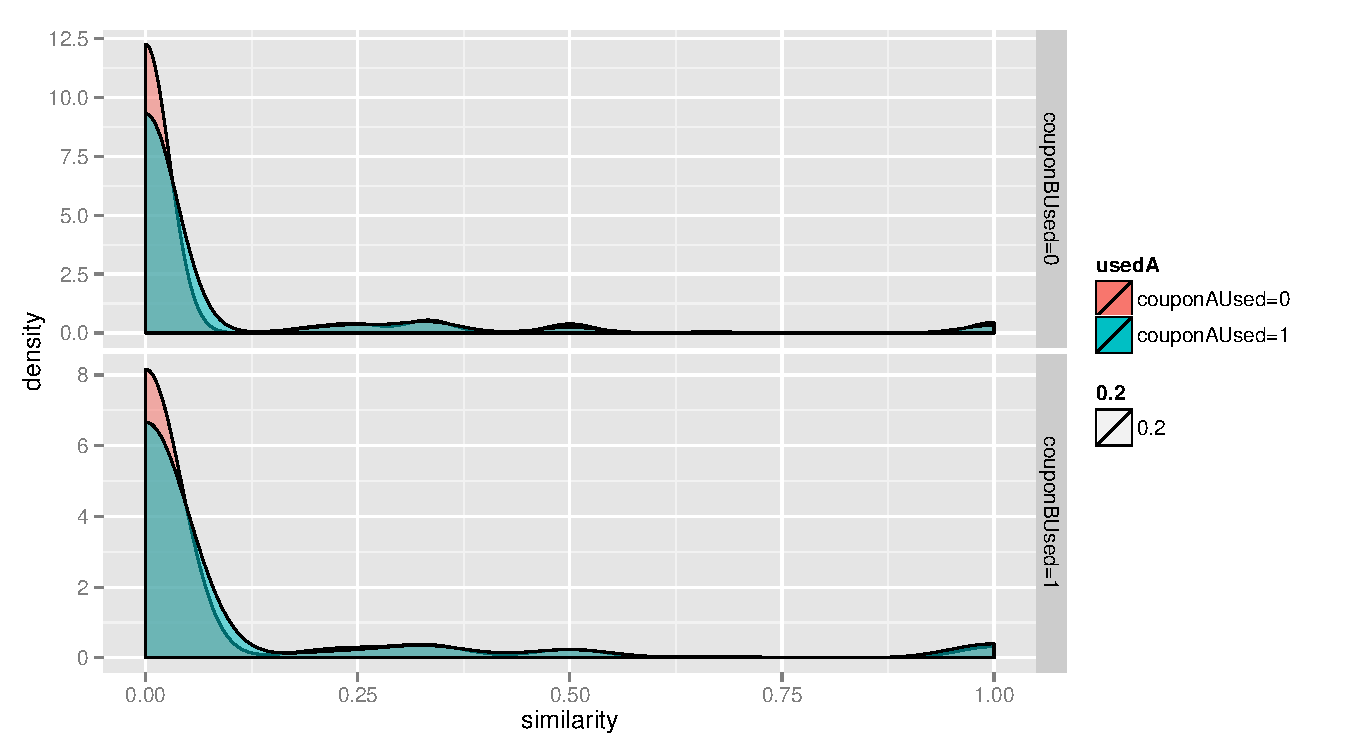
\includegraphics[width=.9\linewidth,height=.9\linewidth]{/Users/user/dmc2015/predictions/graphics/fig_unnamed-chunk-8-1} \end{center}

\end{document}
